% !TEX root = ../main.tex
\newpage
\section{\mywork Mean Field Reductions for undirected graphs}
We will now investigate the questions that were raised after deriving the \MFR. How do we deal with the curse of dimensionality concerning the degree distribution? But there are also other questions to be answered. If the synchronisation dynamics of the network of Theta neurons \eqref{eq:thetaneuronnetwork} can be predicted by the Ott-Antonsen reductions \cref{eq:OttAntonsenSystemFull,eq:OttAntonsenMeanField,eq:MeanField}, then it can also be measured by the order parameter \eqref{eq:orderparameter}. These systems describe the same quantity, but how can we show that?


\subsection{Directed graphs as permutations}
So how can we use the \MFR efficiently when the network is a directed graph with an asymmetrical adjacency matrix? Let's investigate.
\begin{itemize}
\item Sampling $\kinb$ and $\koutb$ from a bivariate distribution requires us to find the marginal distribution of $P$ for $\kinb$, sampling $\kinbi$, and then sampling $\koutbj$ from $P$ while keeping $\kinbi$ fixed. This is a cumbersome process. And what relation would there be between $\kinb$ and $\koutb$?
\item However, if we assume that the marginal distributions for $\kinb$ an $\koutb$ are independent, there is a simplification to be found. We can even assume that the two marginal distributions are identical univariate distributions. 
\item Hence, we can sample $\kinb$ from a univariate distribution and find $\koutb = \permute ( \kinb )$ so that the total number of links remains constant. 
\end{itemize}

This hypothesis can be tested: we assume that $P(\k) = P(\kin) \cdot P(\kout)$ so that $P$ consists of two identical and independent distributions, given by the distributions presented in Chapter \ref{sec:NetworkTopologies}. Then, we sample $\kinb \sim P(\kin)$ and perform a permutation to find all node degrees $\k_j$. The surface given by $P$ and the histogram of $\k_j$ have been plotted in Figure \ref{fig:2Ddistributions}. As we can see, the variates follow the distribution well. 

\begin{figure}[ht]
\centering
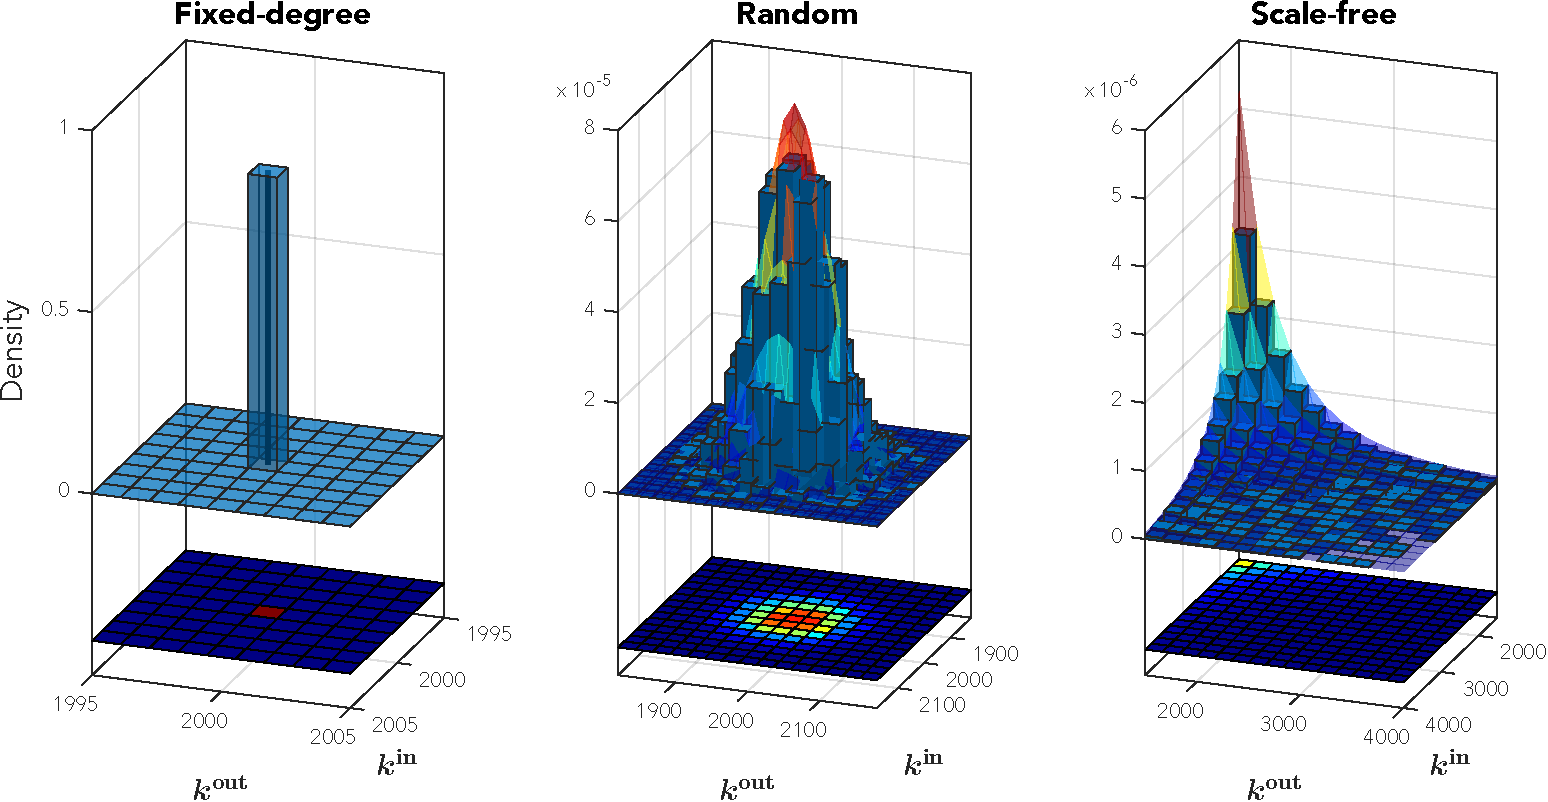
\includegraphics[width = \textwidth]{../Figures/Distributions/2D.pdf}
\caption{Bivariate distributions for different network topologies, using 10$^4$ number of samples. The surface given by $P(\k)$ is well approximated by the histogram of variates sampled from a univariate distribution. $\kmean =  2 \times 10^3$ for all topologies, $p \approx 0.2$ for the random network and $\gamma = 4.3$ for the scale-free network.}
\label{fig:2Ddistributions}
\end{figure}
%Hence, we can use univariate distributions in our simulations of the Ott-Antonsen Mean Field \eqref{eq:OttAntonsenMeanField}.
However, the problem remains the same: $\K$ is too large to simulate the dynamics of the network. What we can do, is use $P(k)$ in the Ott-Antonsen reduction for a symmetric network, and observe how much the dynamics of the asymmetric, simulated network differ.

\subsection{Building the adjacency matrix} \label{sec:buildingA}
If we want to simulate the network of theta neurons \eqref{eq:thetaneuronnetworkcurrent} we need to construct the adjacency matrix. We can find an exact solution for $A$ given the degree vectors in \eqref{eq:definekinkoutfromP}. $A_{ij}$ represents a directed graph, but $A_{ij} \neq A_{ji}$ is not a necessary condition. For the elements of $A_{ij}$ we need to find $N^2$ number of variables. We have the following constraints:
\begin{enumerate}
\item The column- and row-sums of $A_{ij}$ must be equal to $\kinb$ and $\koutb$, see \eqref{eq:definekinkoutfromA}. 2$N$ constraints.
\item Self-coupling is mandatory: $A_{ii} = \boldsymbol{1}$. $N$ constraints.
\item The total number of links is constant: $\sum_{i=1}^{N} \kinbi \equiv \sum_{j=1}^{N} \koutbj \equiv \sum_{i,j=1}^{N}A_{i j}$. 1 constraint.
\end{enumerate}
This means that there are $N^2 - (3N + 1)$ variables to find. Once a solution has been found, $A_{ij}$ can be switched with element $A_{ic}$ if $A_{ij} \neq A_{ic}$ and $A_{rj}$ with $A_{rc}$, which yields a new feasible solution. The number of switches one can make is high, and therefore we can simply try a stochastic approach to obtain $A$:
\begin{enumerate}
\item Choose a random row $i \in [1,N]$. $A_{i,i} = 1$, so we need $m = \kinbi - 1$ elements that are 1.
\item Perform $\permute ( \koutbj, j \neq i)$ and therein find the indices $\boldsymbol{\ell}$ of the $m$ first largest elements. 
\item Set $A_{il} = 1 \: \: \forall \: \: l \in \permuteinv (\boldsymbol{\ell})$.
\end{enumerate}
Algorithms that find the largest value in a vector start from the first or the last element. The permutation allows us to find different maxima every time by shuffling the vector.

\begin{figure}[H]
\centering
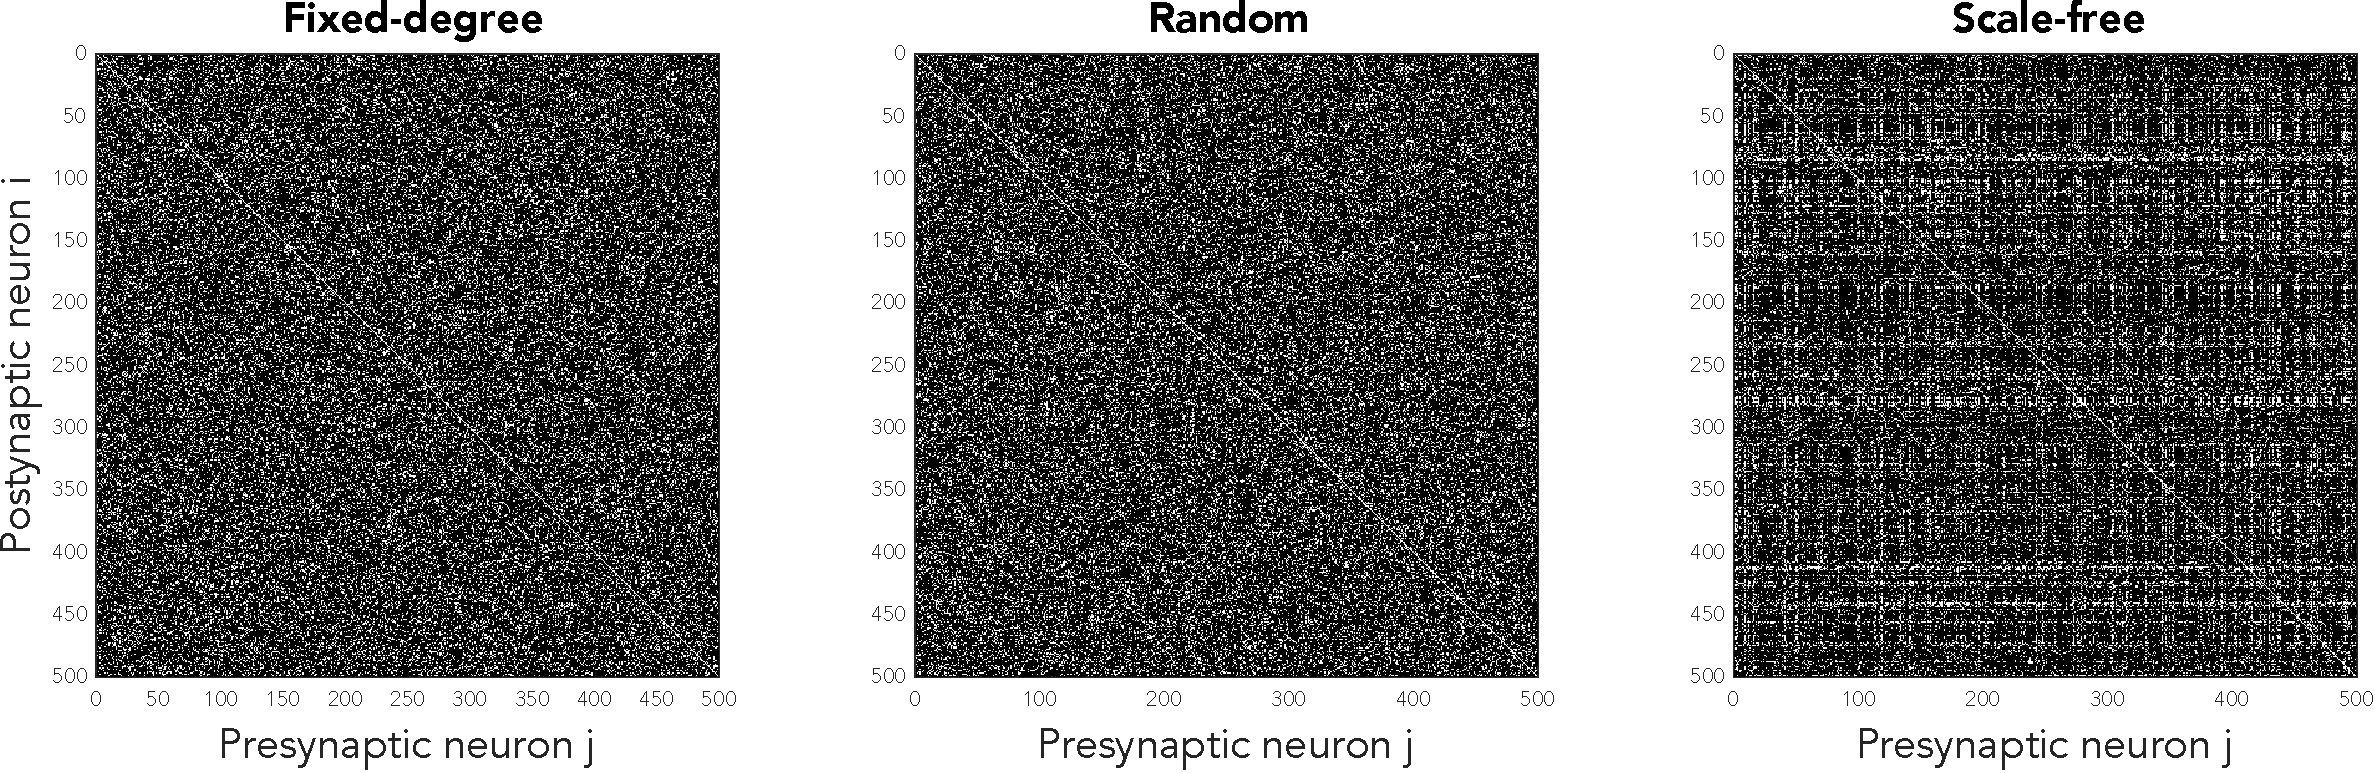
\includegraphics[width = \textwidth]{../Figures/Adjacency_matrices.pdf}
   \caption{Adjacency matrices for different types of networks with $N$ = 500 and $\kmean$ = 100. We can see how the fixed-degree network is quite homogeneous, while the random network shows some more clustering. The scale-free network has a low number of nodes with a very high degree, which is why we see vertical and horizontal stripes in the adjacency matrix.}
   \label{fig:adjacencymatrices}
\end{figure}



\subsection{Initial conditions: analitical versus numerical approaches} \label{sec:initialconditions}
As our goal is to compare theory and simulations, we need to be able to start both at the exact same condition. This notion requires us to transform between the three number sets that our dynamics are described in: $\theta \in \T^N$, $z \in \C^{M_{\k}}$ and $Z, \bar{Z} \in \C$. It is really only necessary to find a transformation that holds accurately for $t=0$, as the distribution of $\theta$ and $z$ over their number set is unknown, but we assume they converge to that distribution when the systems are computed.

%As the systems in \cref{eq:orderparameter,eq:OttAntonsenMeanField,eq:MeanField} describe the same dynamics for fully connected networks, it is important to be able to transform initial conditions between systems. If we expect their behaviour to be the same, then we need to test that by starting from the same point in time. Hence we can test whether \textsl{macroscopically} we can find the same equilibria, but we can also test \textsl{microscopically} whether the systems arrive at those points at the same time. 

%The order parameter \ref{eq:orderparameter} and the mean-field order parameter \eqref{eq:OttAntonsenMeanField} describe the same dynamics for fully connected networks. Testing this hypothesis 

%  If the initial conditions of all systems are exactly the same, then we should find that they describe the exact same behaviour.
% - macroscopically and microscopically - and this is the best way to test the \MFR theory. 

%When transforming between $\theta_i(t) \leftrightarrow z(\k,t) \leftrightarrow Z(t)$ we go from $\T^N \leftrightarrow \C^{M_\k} \leftrightarrow \C$. If we have the same initial conditions, then all systems will predict the same behaviour. We will only map everything to $\C$.\\
As we can optimally study the behaviour of $Z$ and $\bar{Z}$ in the complex unit circle, the most important transformations are those that yield $\theta$ and $z$ from $Z$ and $\bar{Z}$ respectively. Hence, we can start our simulations anywhere in $\C$, close to the limit cycle for example, which was observed in Figure \ref{fig:MFRCPW}.

%As we can study the behaviour of $Z$ and $\bar{Z}$ in the complex unit circle, the most important relation we need to find is the transformation from $\C$ to $\T^{N}$ and from $\C$ to $\C^{M_{\k}}$, which yield the phase angles $\theta_i(0)$ and the degree dynamics $z(\k,0)$ from $Z(0)$ and $\bar{Z}(0)$ respectively. \\

% The following maps can be used to transform the initial conditions, but as they do not give any qualitative information on the dynamics or distributions of the variables, they are not valid for transforming between dynamics. \\

Let us start with the simplest transformation. Given an initial phase angle $\theta_i(0)$ or initial degree dynamics $z(\k, 0)$ we wish to find their resulting description in the complex unit circle. Mapping operations onto the order parameter is straightforward using \eqref{eq:orderparameter} and \eqref{eq:OttAntonsenMeanField}:
\begin{align}
\theta_i(0) \xrightarrow{\hspace*{8mm}} Z(0) &= \frac{1}{N} \sum_{j=1}^N e^{\ic\theta_j(0)} \label{eq:thetatoZ}\\
z(\k,0) \longrightarrow \bar{Z}(0) &= \frac{1}{N} \sum_{\k \in \K} P(\k) z(\k, 0)  \label{eq:ztoZ}
\end{align}
Here we can immediately see that information about the distribution of $\theta$ and $z$ is lost when taking the (weighed) average. 

Starting from an initial synchronization $Z(0)$ and taking the inverse tranfsormation, we can make use of the fact that the average of a set of identical values is the value itself. This is simple for $\theta_i(0)$: we can take all phase angles to be the same at $t = 0$. For $z(\k,0)$ we have a weighed average which we need to undo, while making sure that the whole sums up to $N$ by multiplying with the total number of neurons $n(\k)$ of degree $\k$:
\begin{align}
Z(0) \xrightarrow{\hspace*{8mm}} \theta_i(0) &= -\ic \cdot \log \left( Z(0) \right)  \label{eq:Ztotheta} \\
Z(0) \longrightarrow z(\k,0) &= \frac{Z(0) \cdot n(\k)}{P(\k)} \label{eq:Ztoz}
\end{align}
This approach only alters the magnitude of $Z(0)$, so that $z(\k,0)$ will be distributed on a line through $Z(0)$. Then, transforming between $\theta_i$ and $z(\k)$, we need to filter $\theta_i$ per degree as there exist $n(\k)$ number of nodes with $\degree ( \theta_i ) = \k$:
\begin{alignat}{2}
z(\k,0) \longrightarrow \theta_i(0) &= -\ic \cdot \log \left( \frac{z(\k)\cdot P(\k)}{n(\k)} \right) \qquad &&\forall \: \theta \in \{ \theta \: | \: \degree(\theta) = \k \}  \label{eq:ztottheta}\\
\theta_i(0) \longrightarrow z(\k,0) &= \sum_{\k} e^{\ic \vartheta_{\k}} \qquad \qquad &&\forall \: \vartheta_{\k} \in \{ \vartheta_{\k} = \sum^{n(\k)} \theta \: | \: \degree(\theta) = \k \} \label{eq:thetatoz}
\end{alignat}
%We can see how $\lim_{N \rightarrow +\infty} n(\k) = P(\k)$, which makes these maps exact for any network size. 
%The reason that these transformations can only hold for the initial state is because it is currently unknown what distributions $\theta_i(t)$ and $z(\k,t)$ should have. That information is lost when taking the (weighed) average in \eqref{eq:orderparameter} and \eqref{eq:MeanField}. \\

The relations derived here raise problems when $P(\k)$ spans different orders of magnitude. \eqref{eq:ztoZ} does not bound $z$ to its set, so it might occur that the distribution of $z$ has values outside of the complex unit circle. However, transforming back to $\bar{Z}$ will always be correct. This problem does not occur for $\theta$, as $\T$ is a one-parameter group. Let us look at the example in Figure \ref{fig:mappings}, where we are trying to find $z(\k, 0)$ so that $\bar{Z}(0)$ is equal to the desired initial condition $Z(0) = $ -0.2 + $\ic$0.8, using a scale-free topology. \\

%The initial values of $z$ are not bound on $\C$, so it might occur that the initial condition given through \eqref{eq:ztoZ} is exact, but that the distribution of $z(\k,t)$ leaves us with some out of the complex unit circle. Let us look at the example in Figure \ref{fig:mappings}, where we are trying to find $z(\k, 0)$ so that $\bar{Z}(0)$ is equal to our desired initial condition $Z(0) = $ -0.2 + $\ic$0.8. \\

% Especially for scale-free networks, where there is a large difference between the smallest and largest degree, this offset is large
 
When simply taking all $z(\k, 0) = Z(0)$, there is a slight offset between $Z(0)$ and $\bar{Z}(0)$. However, the dynamics are well-behaved and the end-state is almost a smooth curve. One can really interpret this curve as the attractive manifold of the Ott-Antonsen reduction. This method is an easy way of quickly coming up with an initial condition, without requiring any computation. In general, this yields quite a good approximation. \\

When using \eqref{eq:ztoZ}, we can see that the initial conditions lie on a straight line through the origin indeed, and that $\bar{Z}(0)$ is exactly equal to $Z(0)$. When a given $\k$ yields a small $P(\k)$, $z(\k,0)$ will be scaled away from the origin. This means that the dynamics of nodes of that degree are not a good representation. However, their contribution to $\bar{Z}$ in \eqref{eq:OttAntonsenMeanField} is small, so sometimes these effects cancel out and the dynamics are in fact quite smooth. However, we can see that in our example the dynamics are not represented well, resulting in large errors after conception and a more random end-state. We do expect these effects to cancel out after longer periods and for larger $N$, as the manifold is attractive and larger networks cancel out outliers, but our aim is to be as precise as possible from $t=0$. \\

\begin{figure}[H]
\centering
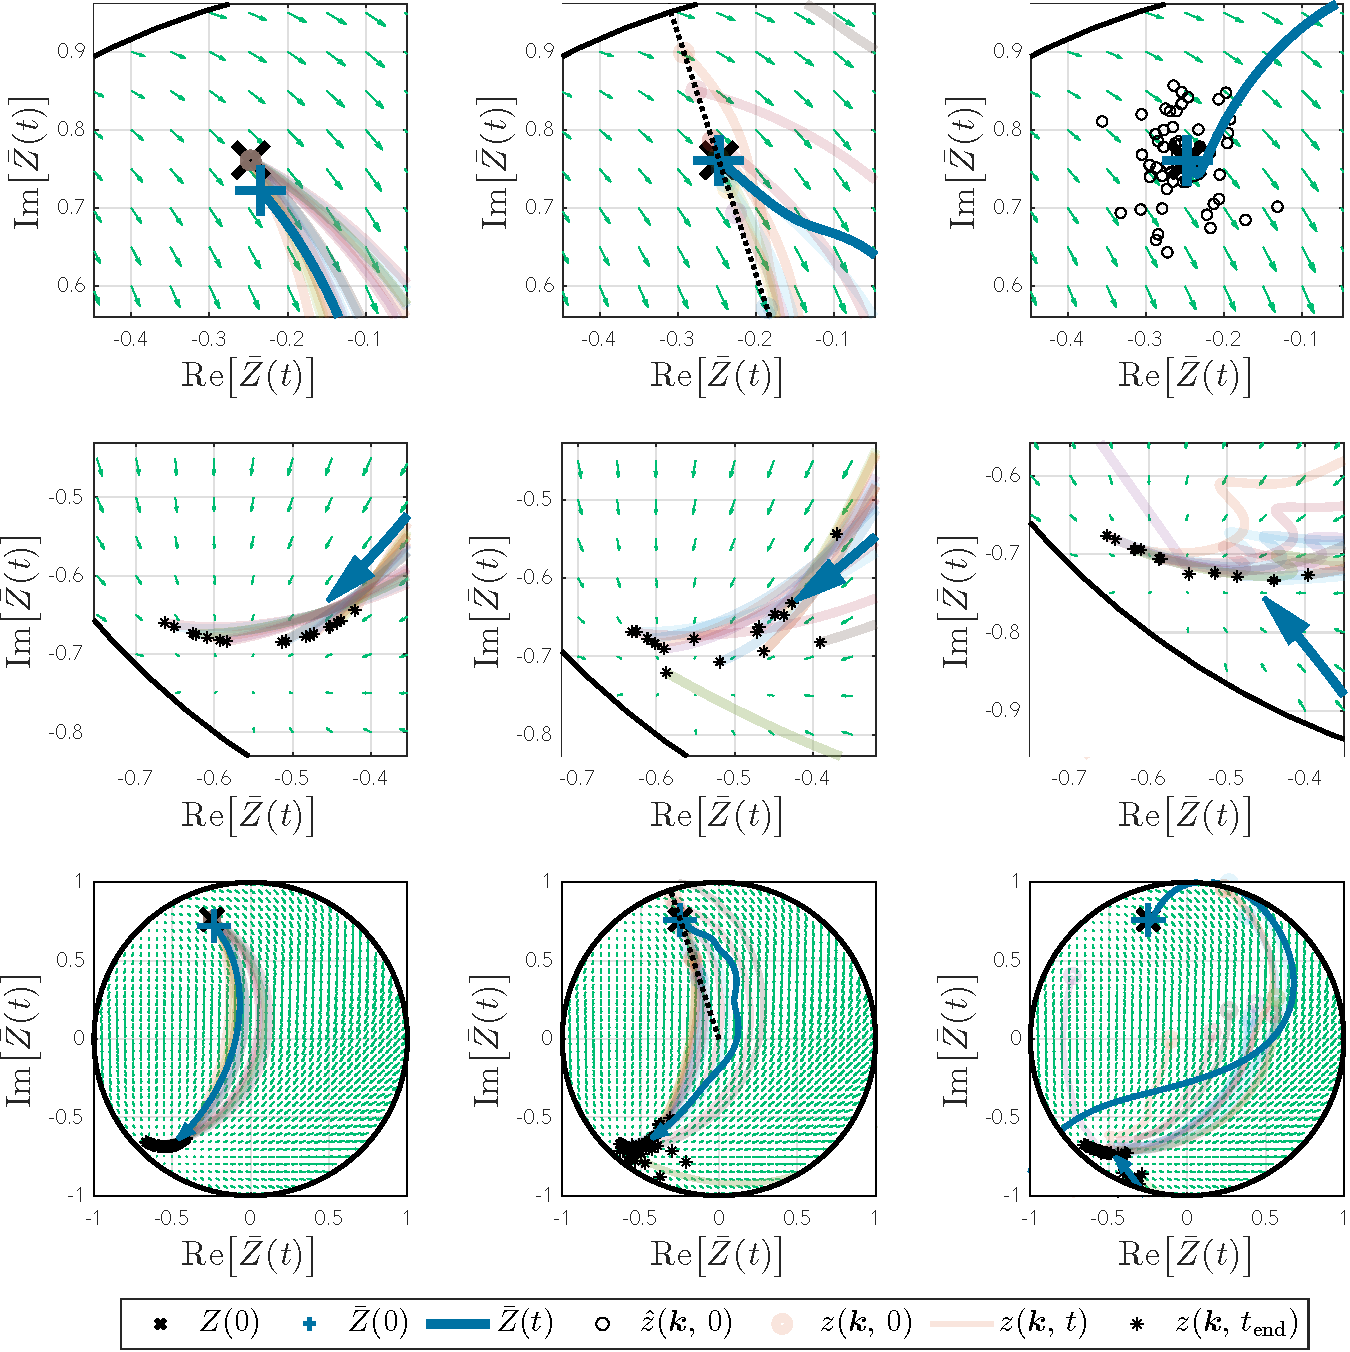
\includegraphics[width = \textwidth]{../Figures/PhaseSpace/Mappings.pdf}
   \caption{Simulation of 1000 neurons in a scale-free network. Example on the importance of accurate initial conditions. A scalefree network is used to show the outcome of different strategies of }
   \label{fig:mappings}
\end{figure}

When trying to address the problems that are encountered here, we can try and find the distribution of $z(\k,0)$ numerically by solving for the root of $f(z) = \| Z(0) - \bar{Z}(0) \|$ (where $\bar{Z}$ is computed from $z$) under the constraint that $| z | \leq 1$, starting from an initial guess $\hat{z}$, clustered around $Z(0)$. The resulting initial distribution is quite clustered but as it is mostly a result of the constraint, we are more interested in the end-state, which shows a lot of improvements. The initial conditions are exact (up to $10^{-6}$) and the dynamics are smooth, which makes this method the most desirable. However, convergence can be very slow for scale-free networks, and the complexity of the system to solve scales with $\sim N^2$ . It is therefore necessary to judge which method to use when performing a new simulation.


\subsection{Commutativity of complex vectors} 
It is important to notice that in \eqref{eq:OttAntonsenSystemFull} and \eqref{eq:OttAntonsenMeanField} and many other equations in this work, we compute an inner vector product, which is non-commutative for complex numbers:
\begin{align}
a \cdot b = \overline{b \cdot a} \qquad a, b \in \C^r
\end{align}
This is the result of the \textsl{Conjugate} or \textsl{Hermitian} symmetry of the inner product. This is especially important in the \matlab implementation, as one needs to remain consistent with left-hand or right-hand products.



\subsection{Fixpoint iteration}
In \cite{OttAntonsen2017} a fixpoint iteration is suggested to find attractive fixpoints of the system \eqref{eq:OttAntonsenSystemFull}. If we set $\frac{\partial z(\k, t)}{\partial t} = 0$ we can solve the following system:
\begin{align}
\ic \frac{(z(\k, t)-1)^{2}}{2} &= \frac{(z(\k, t)+1)^{2}}{2} \cdot I(\k) \nonumber \\
\ic \left(\frac{z(\k, t)-1}{z(\k, t)+1}\right)^2 &= I(\k) \nonumber \\
\frac{z(\k, t)-1}{z(\k, t)+1} &\equiv b(\k,t) \nonumber \\
z(\k, t) - 1 &= b(\k,t) z(\k, t) + b(\k,t)  \nonumber \\
z(\k, t) \cdot (1 - b(\k,t)) &= b(\k,t)  + 1\nonumber
\end{align}
We can then obtain the stable equilibria from:
\begin{align}
\ic b(\k,t)^2 = I(\k) \hspace{10mm} z(\k, t)_{\pm} = \frac{1 \pm b(\k,t)}{1 \mp b(\k,t)} \label{eq:fixedpointiterations} 
\end{align}
where the signs are chosen so that $\vert z(\k, t) \vert \leq 1$. This works well, and in general this method converges fast.


\subsection{A Newton-Raphson iteration for all fixpoints}
The fixpoint iteration \eqref{eq:fixedpointiterations} only gives us the stable equilibria of the \MFR. We can obtain all equilibria and their stability through the Jacobian from a Newton-Raphson iteration, which has been described in \ref{app:NewtonRaphson}. However, finding the Jacobian is a challenge, as \eqref{eq:OttAntonsenSystemFull} is non-holomorphic: $H_2(\k,t)$ does not satisfy the Cauchy-Riemann equations.
%For \eqref{eq:OttAntonsenSystemFull}, we can compute the Jacobian for the diagonal and off-diagonal elements separately. But as $z(\k,t)$ is a complex function, first we need to understand what the derivative of a complex function is. 
\begin{align*}
z(\k,t) &= x(\k,t) + \ic \cdot y(\k,t) \qquad x, y \in \R^{M_{\k}}\\
f\left( z(\k,t) \right) &= u\left(x(\k, t), y(\k, t) \right) + \ic v\left(x(\k, t), y(\k, t) \right)\\
&= \frac{1}{\kmean} \sum_{\kacc} P\left(\kacc\right) a\left(\kacc \rightarrow \k\right) \cdot \left( 1 + \frac{z(\kacc, t)^2 + \bar{z}(\kacc, t)^2}{6} - \frac{4}{3} \Re(z(\kacc, t)) \right)\\
&= \frac{1}{\kmean} \sum_{\kacc} P\left(\kacc\right) a\left(\kacc \rightarrow \k\right) \cdot \left( 1 + \frac{x(\kacc, t)^2}{3} - \frac{4}{3} x(\kacc, t) \right)
\end{align*}
This leaves us with only $u$ defined as a real-valued function, so that the Cauchy-Riemann equations do not hold as $v$ is zero. This is tricky, as expressing the Jacobian as a $M_{\k} \times M_{\k}$ matrix of complex numbers reduces the complexity. \\

\textcolor{red}{QUESTION}: \textsl{explain how the Jacobian can be found as a $2 M_{\k} \times 2 M_{\k}$ matrix by using $z(\k,t) = [ x(\k,t), \: y(\k,t)]$ and interweaving the $x$ and $y$ dimension in the matrix, see \cite{Cross2018}. This has been implemented but only stable results for the \PSR state. Right now I still can only find attractive fixpoints. Should I continue on this?}

\subsection{Fixed-degree networks as a baseline}
Now we have all the necessary tools to simulate networks of theta neurons. First, we will use a fixed-degree network, as this is the most simple instance of the different topologies. The results are shown in Figure \ref{fig:InspectMeanFieldFixedDegree}.
There are small differences between simulation and theory, but these are most likely due to a finite network size and a finite integration step. As a matter of fact, the systems \eqref{eq:OttAntonsenMeanField} and \eqref{eq:MeanField} yield the exact same behaviour. This test benchmarks the lowest amount of error we can observe between simulation and theory, as for fixed-degree networks \eqref{eq:OttAntonsenSystemFull} consists of a single equation.
\begin{figure}[H]
\centering
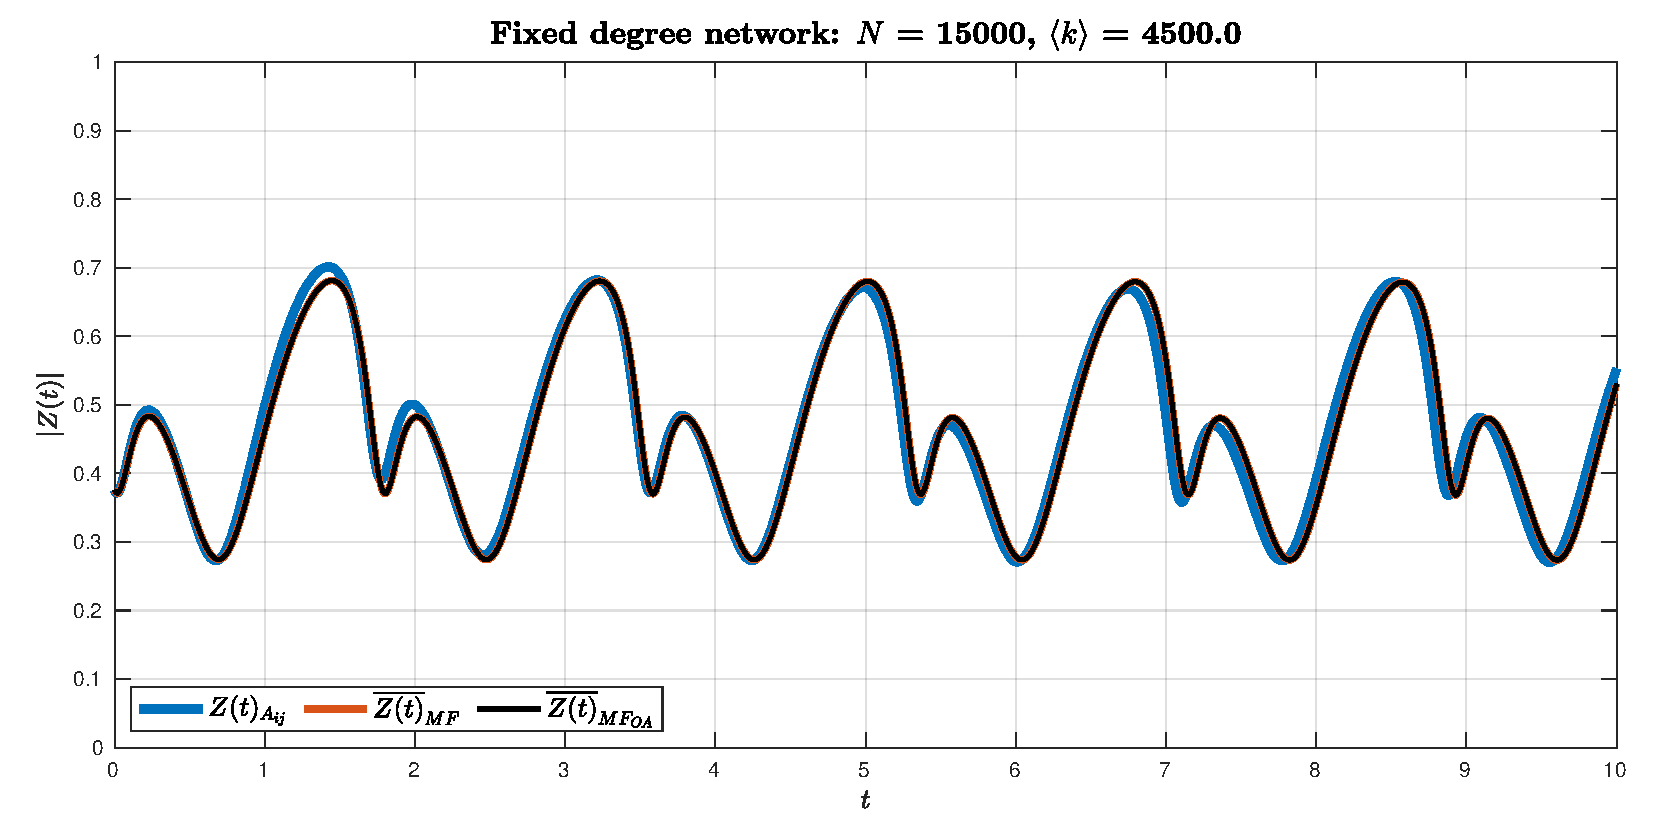
\includegraphics[width = \textwidth]{../Figures/InspectMeanFieldFixedDegree.pdf}
\caption{Comparison of the simulation of a fixed-degree network of Theta neurons and the Ott-Antonsen theory by the magnitude of the order parameter. We see that the same three macroscopic states are found by the three descriptions.}
\label{fig:InspectMeanFieldFixedDegree}
\end{figure}


\subsection{Results for arbitrary network topologies}
The dynamics of random networks seem to be very similar to fixed-degree networks, when looking at the unit circle. We can see in Figure \ref{fig:MFOARCPW_random} that the limit cycle is a little larger. When looking at the dynamics over time the results in Figure \ref{fig:InspectMeanFieldRandom} are also consistent, with a little more deviation between simulation and theory in the \CPW state.

\begin{figure}[H]
\centering
\begin{subfigure}[b]{0.32\linewidth}
   \centering
  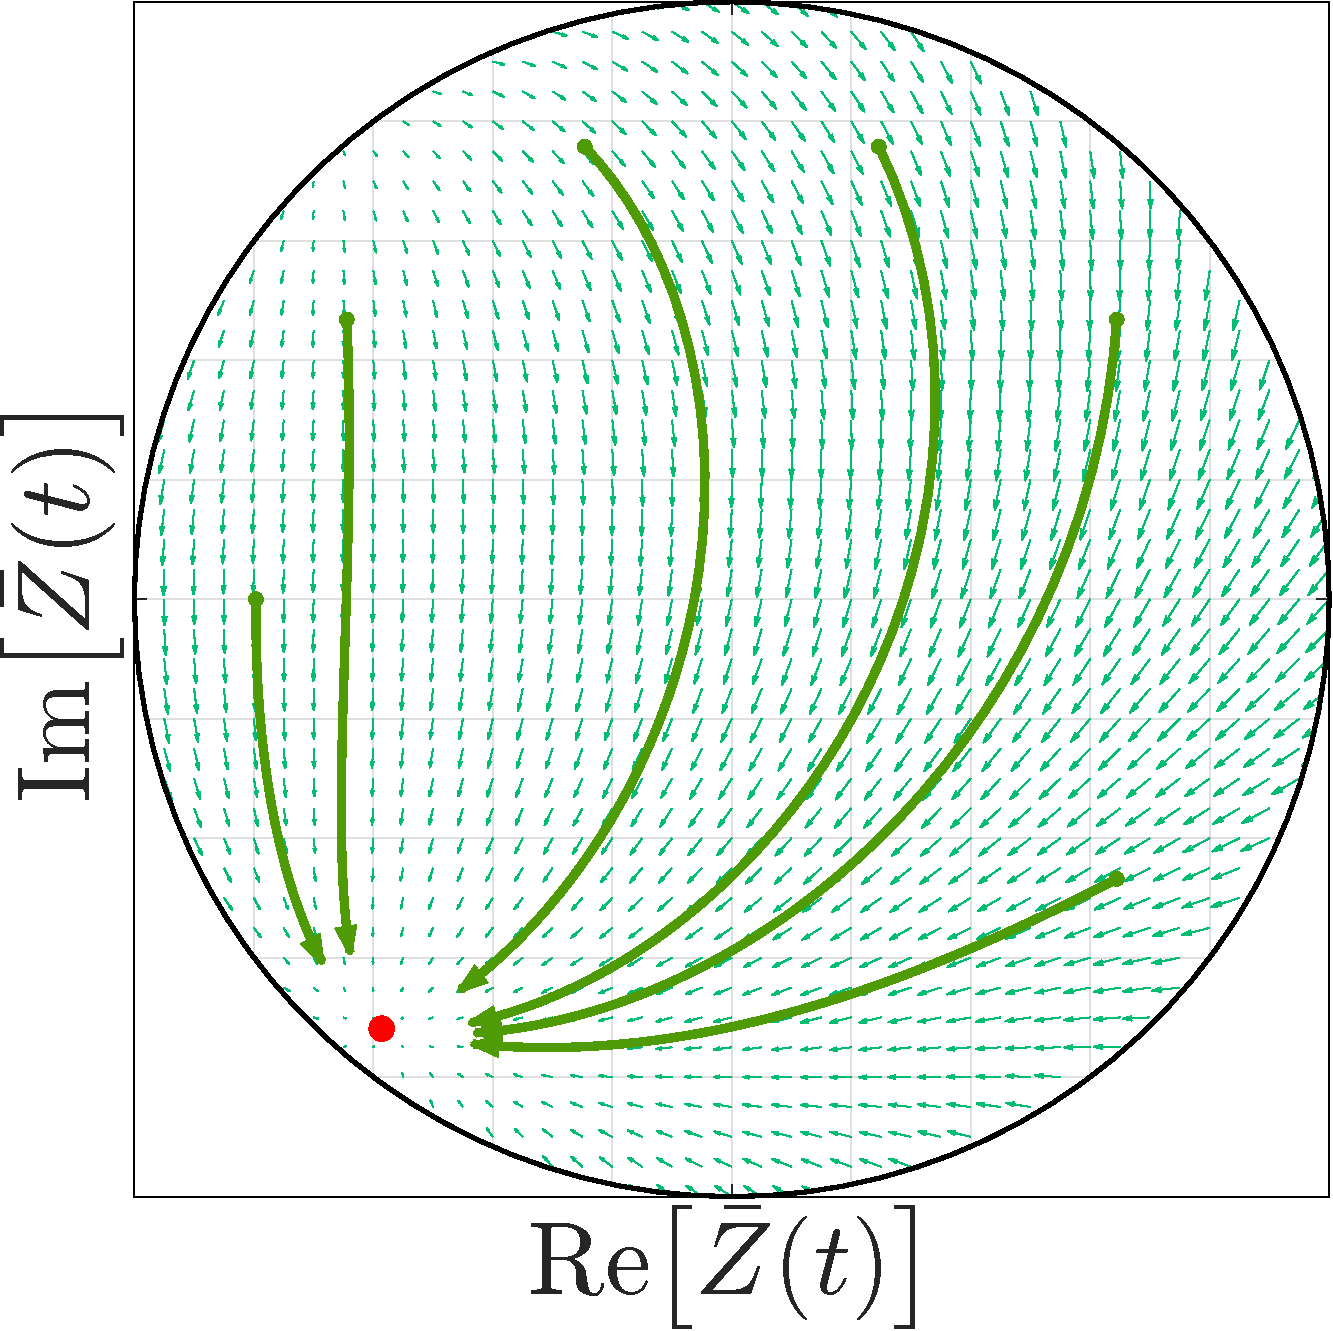
\includegraphics[width=\linewidth]{../Figures/PhaseSpace/MFOARPSR_random.pdf}
   \caption{PSR state for $\eta_0 = -0.9, \sigma = 0.8$ and $\kappa= -2$. The mean field settles onto a stable node.}
   \label{fig:MFOARPSR_random} 
\end{subfigure} \hfill
\begin{subfigure}[b]{0.32\linewidth}
   \centering
  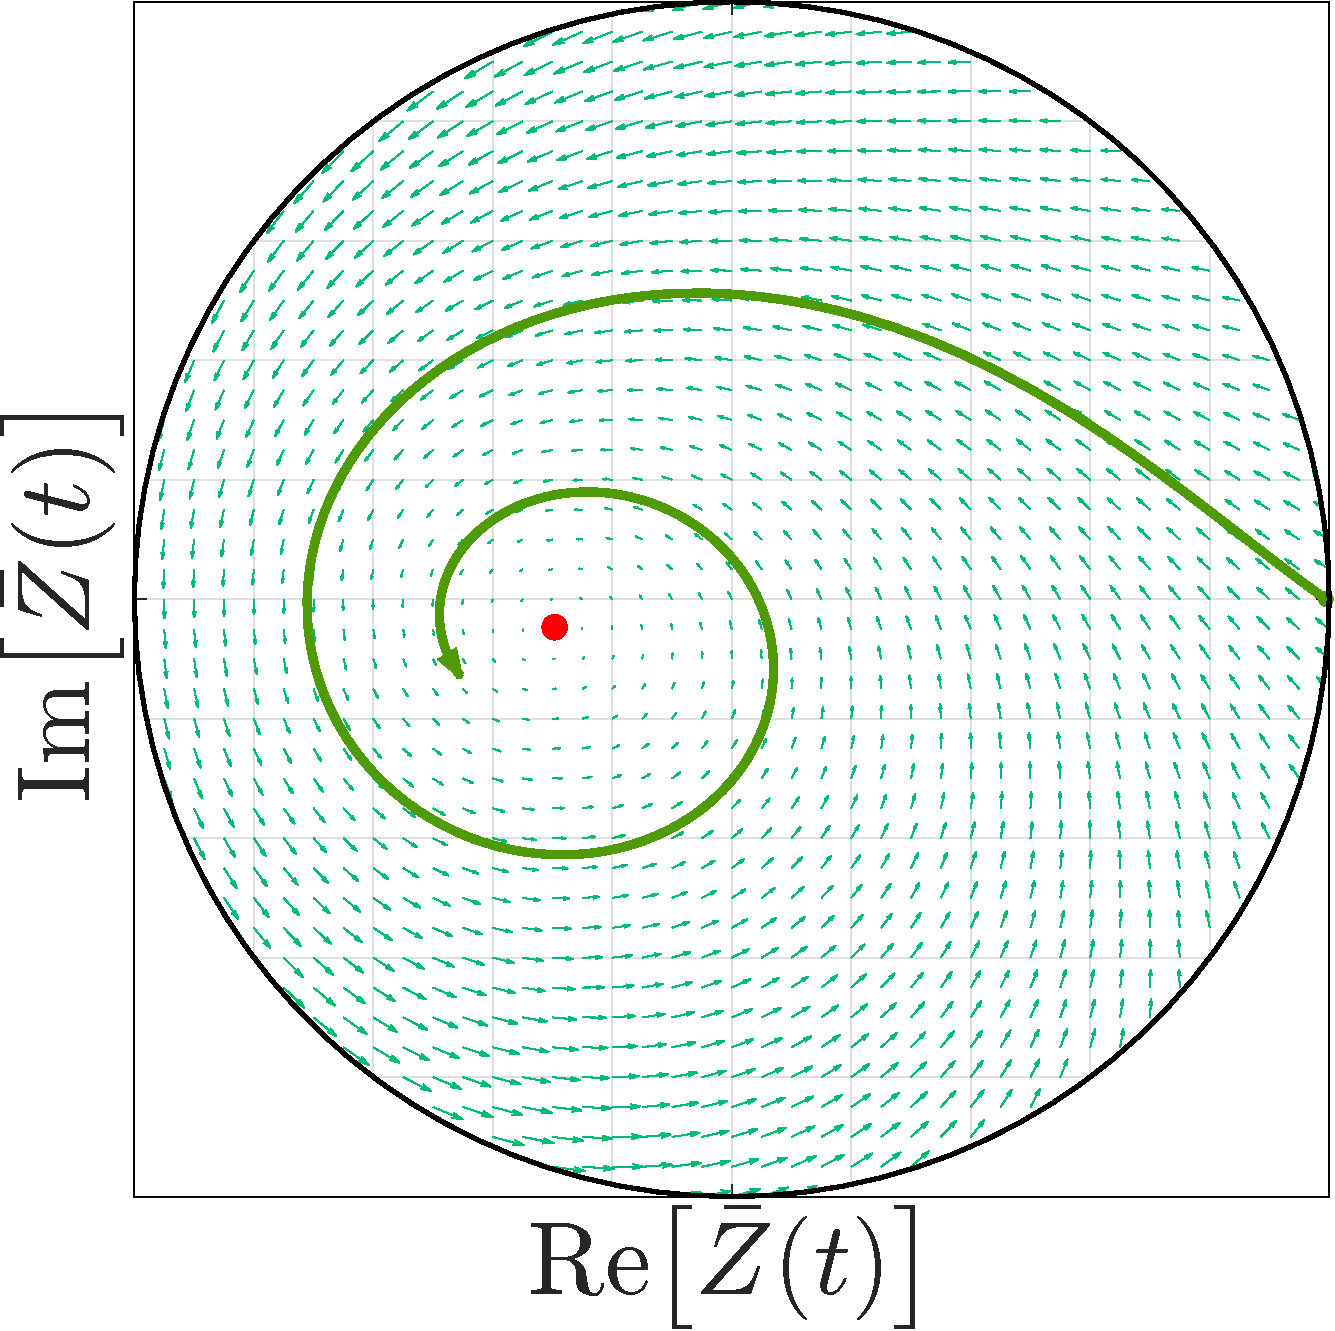
\includegraphics[width=\linewidth]{../Figures/PhaseSpace/MFOARPSS_random.pdf}
   \caption{PSS state for $\eta_0 = 0.5, \sigma = 0.7$ and $\kappa= 2$. The mean field settles onto a stable focus.}
   \label{fig:MFOARPSS_random}
\end{subfigure} \hfill
\begin{subfigure}[b]{0.32\linewidth}
   \centering
  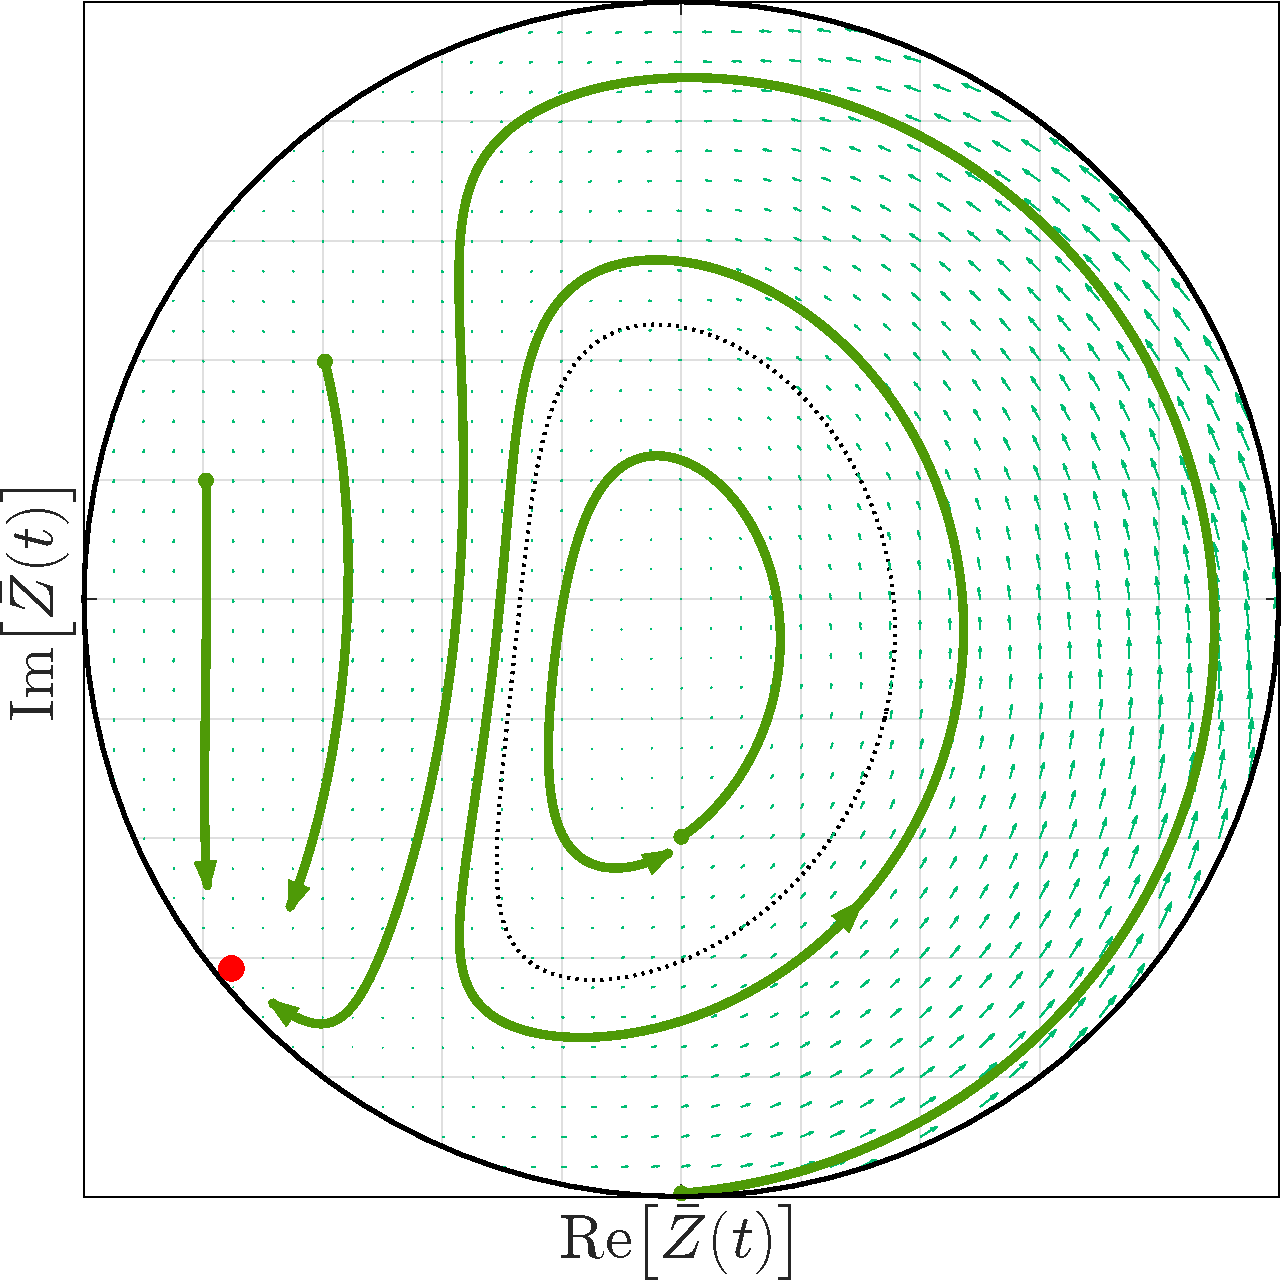
\includegraphics[width=\linewidth]{../Figures/PhaseSpace/MFOARCPW_random.pdf}
   \caption{CPW state for $\eta_0 = 10.75, \sigma = 0.5$ and $\kappa= -9$. The mean field settles onto a stable limit cycle.}
   \label{fig:MFOARCPW_random}
\end{subfigure}
   \caption{Three macroscopic states observed in the \MFR inside the imaginary unit circle $|Z(t)| = 1$. Green arrows mark the phase space vector field and blue trails mark solution curves. Red points indicate equilibrium points, with black arrows marking the direction of the eigenvectors in that point, scaled according to the magnitude of the corresponding eigenvalues. The dotted line in the \CPW state is the limit cycle of the fixed-degree networks, added for reference.}
   \label{fig:macroscopicstatesrandomnetworks}
\end{figure}

\begin{figure}[H]
\centering
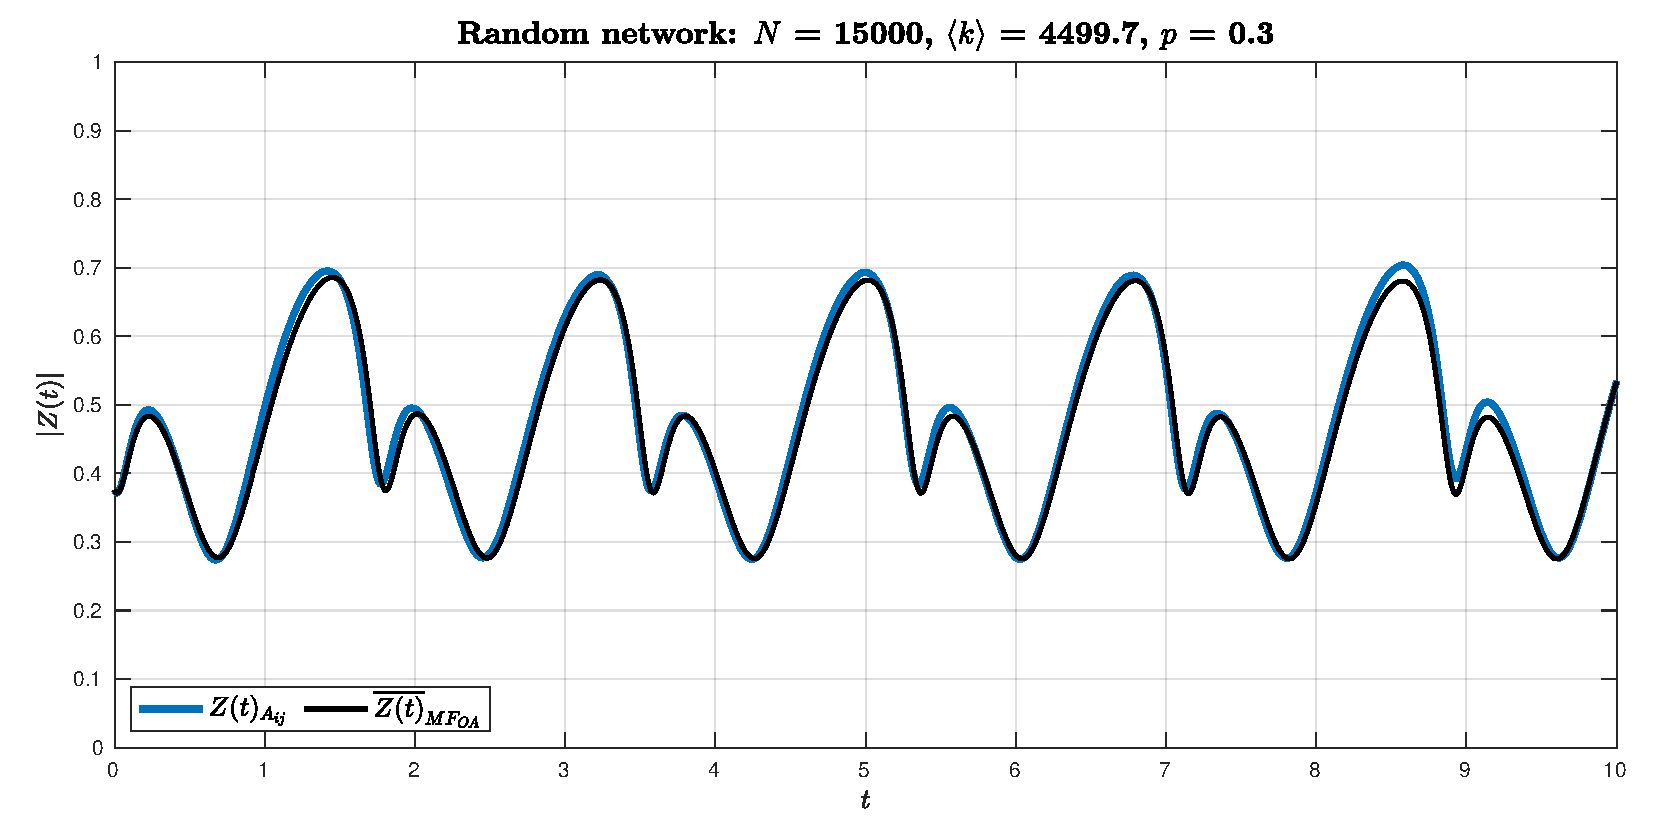
\includegraphics[width = \textwidth]{../Figures/InspectMeanFieldRandom.pdf}
\caption{Comparison of the simulation of a random network of Theta neurons and the Ott-Antonsen theory by the magnitude of the order parameter. }
\label{fig:InspectMeanFieldRandom}
\end{figure}

For scale-free networks, we can see that again the three macroscopic states continue to exist, Figure \ref{fig:macroscopicstatesscalefreenetworks}. However, it seems like there is a fairly large discrepancy between simulation and theory, in Figure \ref{fig:InspectMeanFieldScaleFree}. The stable node in the \PSR state is found at different locations, and the limit cycle in the \CPW state seems to be very different, but with a similar period. Indeed, if we look at the limit cycle to which the dynamics are attracted to in Figure \ref{fig:InspectMeanFieldScaleFreePhaseSpace} we can indeed see two distinct cycles. \\

\textcolor{red}{TODO}: \textsl{argue why this is the case, suspicions on the assortativity function not being assortative.}


\begin{figure}[H]
\centering
\begin{subfigure}[b]{0.32\linewidth}
   \centering
  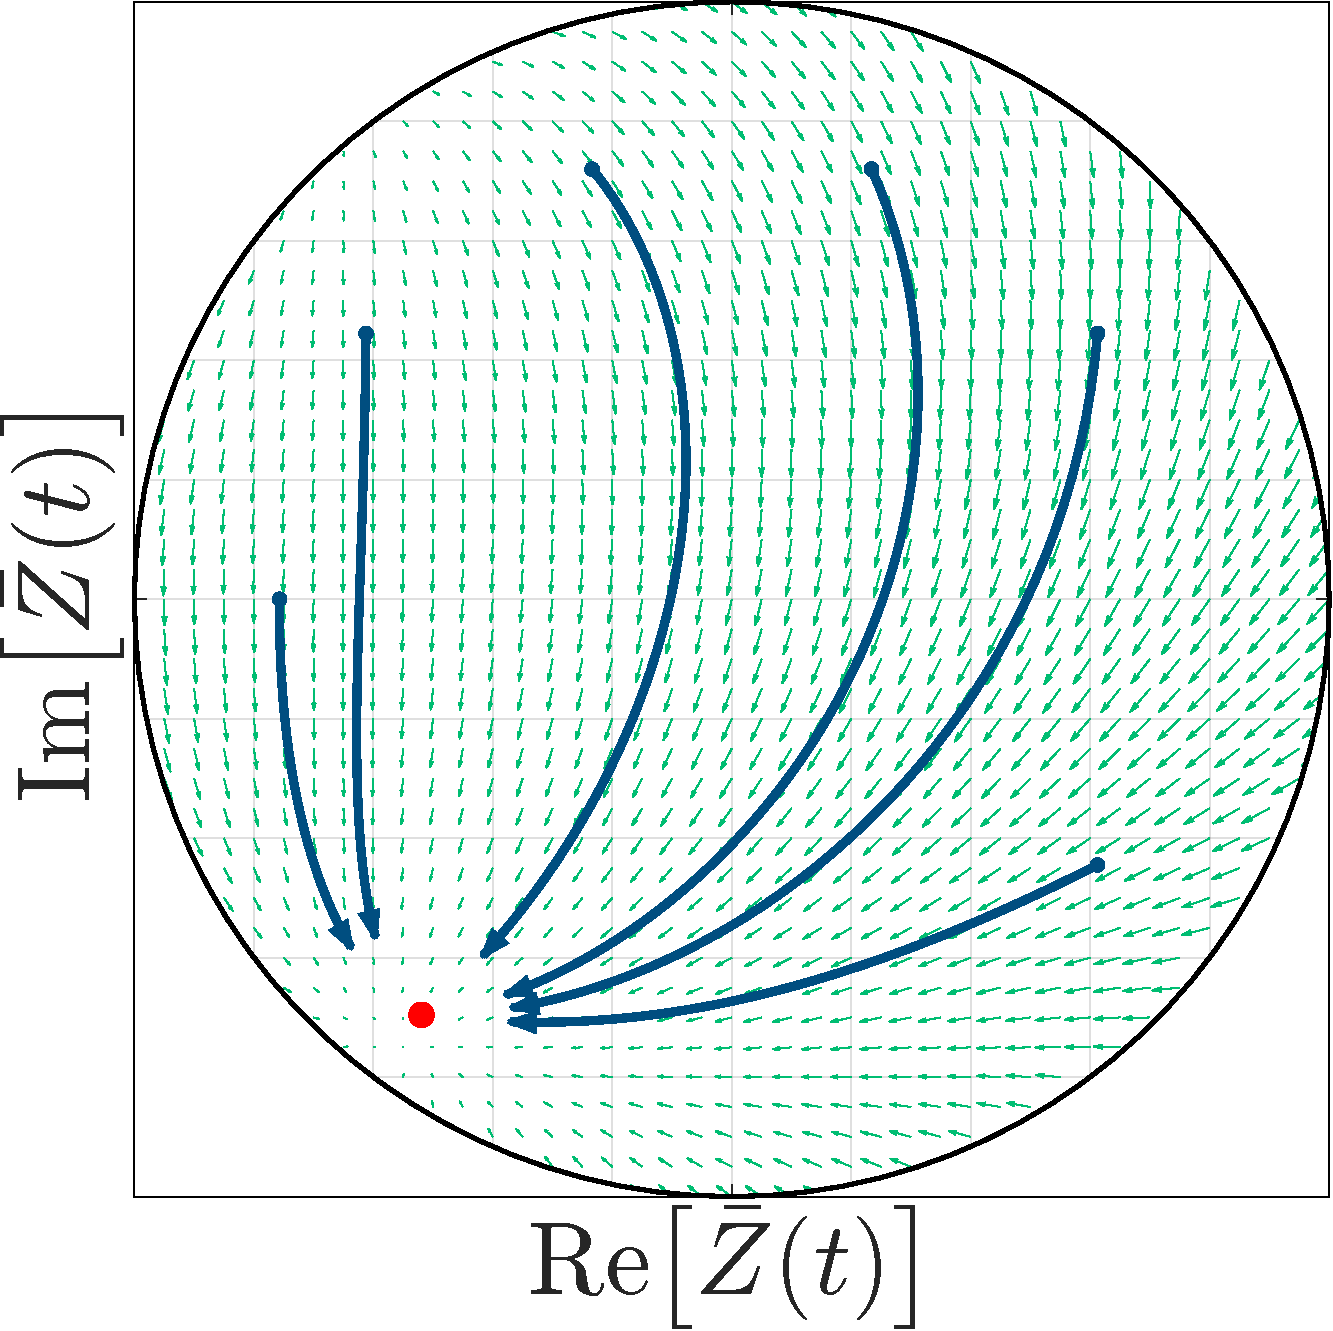
\includegraphics[width=\linewidth]{../Figures/PhaseSpace/MFOARPSR_scalefree.pdf}
   \caption{PSR state for $\eta_0 = -0.9, \sigma = 0.8$ and $\kappa= -2$. The mean field settles onto a stable node.}
   \label{fig:MFOARPSR_random} 
\end{subfigure} \hfill
\begin{subfigure}[b]{0.32\linewidth}
   \centering
  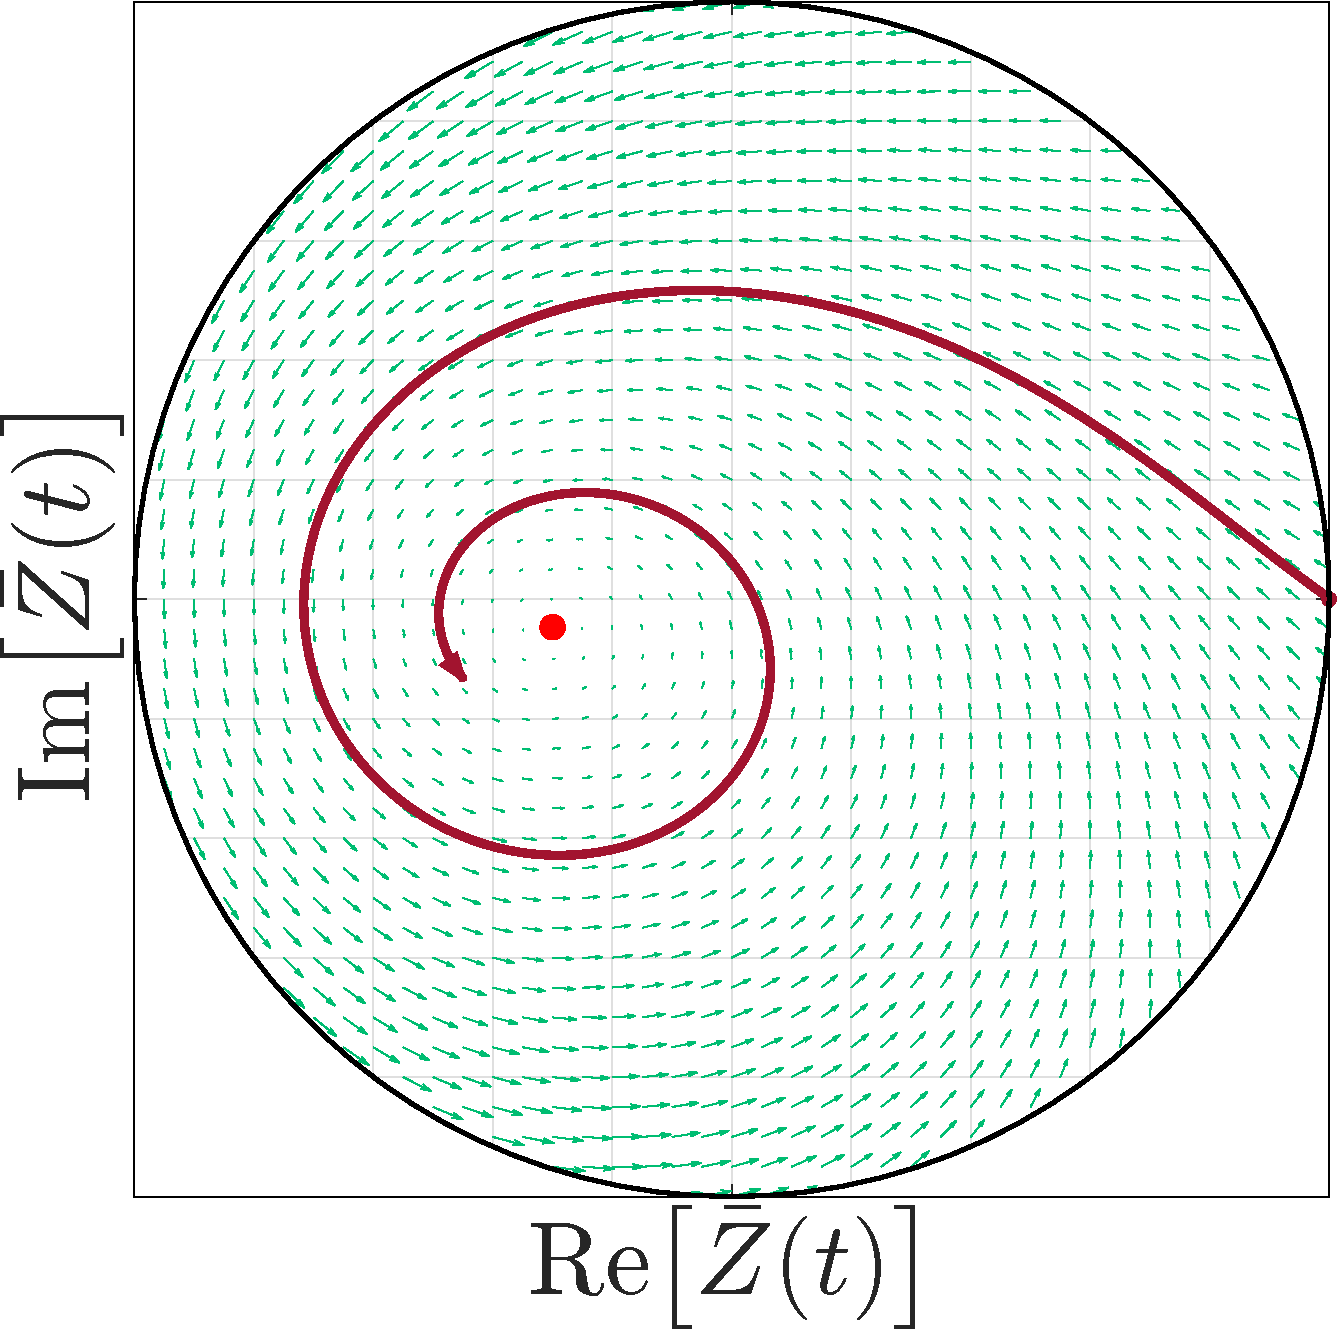
\includegraphics[width=\linewidth]{../Figures/PhaseSpace/MFOARPSS_scalefree.pdf}
   \caption{PSS state for $\eta_0 = 0.5, \sigma = 0.7$ and $\kappa= 2$. The mean field settles onto a stable focus.}
   \label{fig:MFOARPSS_random}
\end{subfigure} \hfill
\begin{subfigure}[b]{0.32\linewidth}
   \centering
  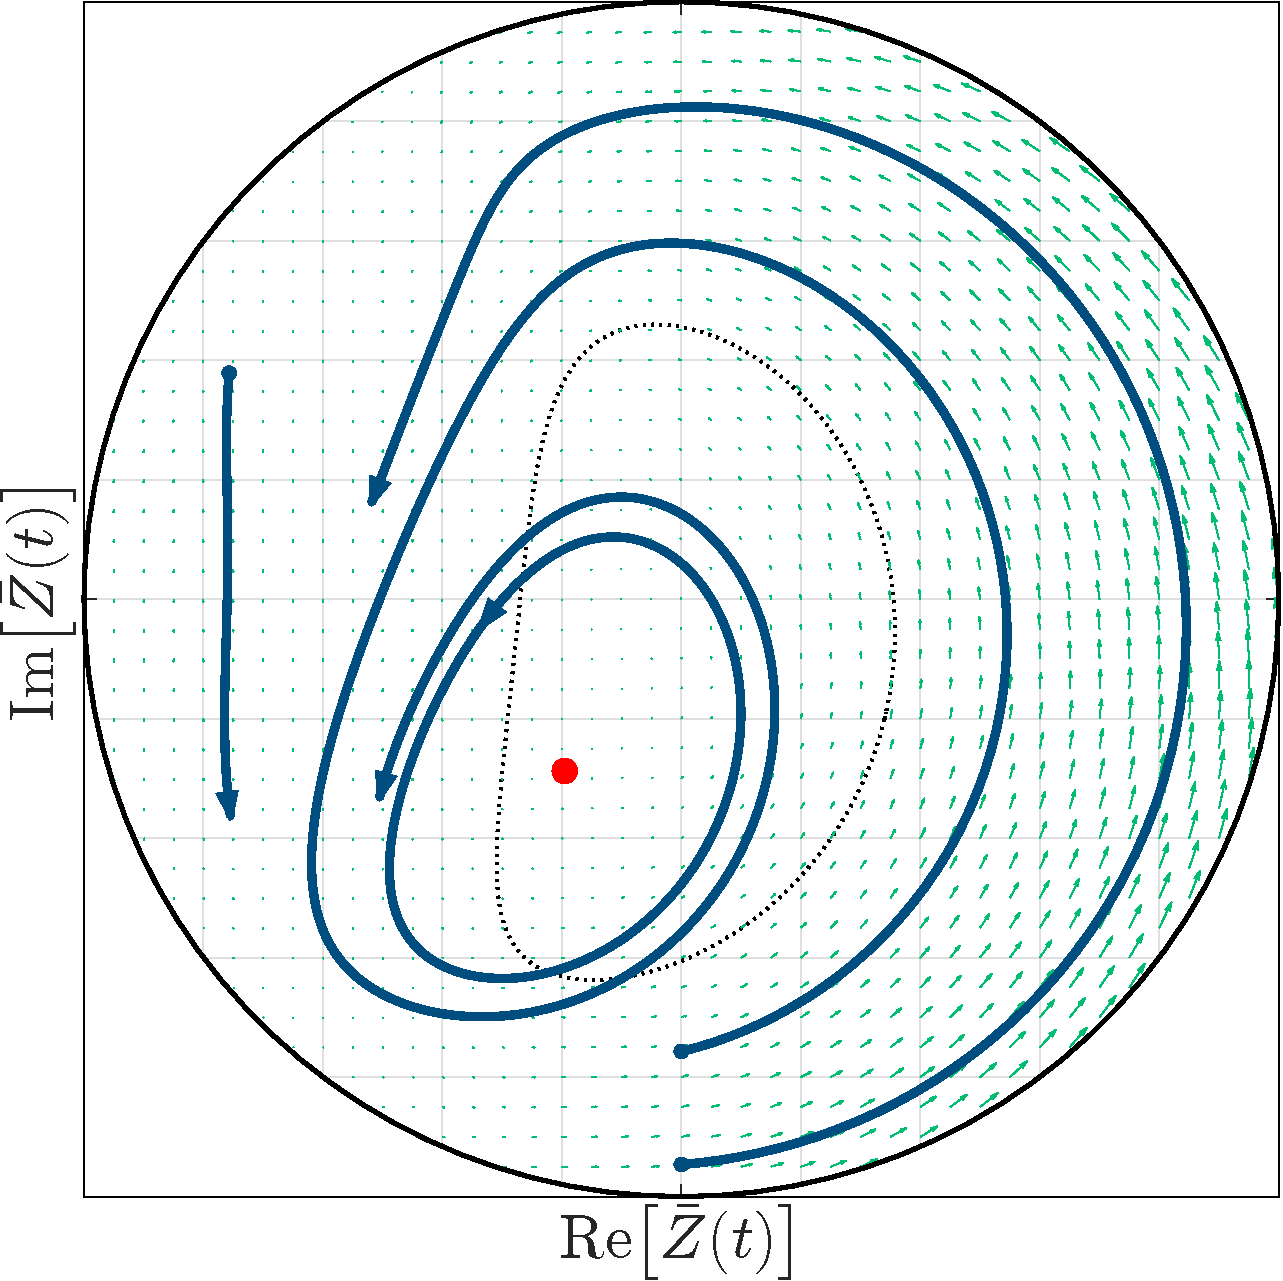
\includegraphics[width=\linewidth]{../Figures/PhaseSpace/MFOARCPW_scalefree.pdf}
   \caption{CPW state for $\eta_0 = 10.75, \sigma = 0.5$ and $\kappa= -9$. The mean field settles onto a stable limit cycle.}
   \label{fig:MFOARCPW_random}
\end{subfigure}
   \caption{Three macroscopic states observed in the \MFR inside the imaginary unit circle $|Z(t)| = 1$. Green arrows mark the phase space vector field and blue trails mark solution curves. Red points indicate equilibrium points, with black arrows marking the direction of the eigenvectors in that point, scaled according to the magnitude of the corresponding eigenvalues. The dotted line in the \CPW state is the limit cycle of the fixed-degree networks, added for reference.}
   \label{fig:macroscopicstatesscalefreenetworks}
\end{figure}

\begin{figure}[H]
\centering
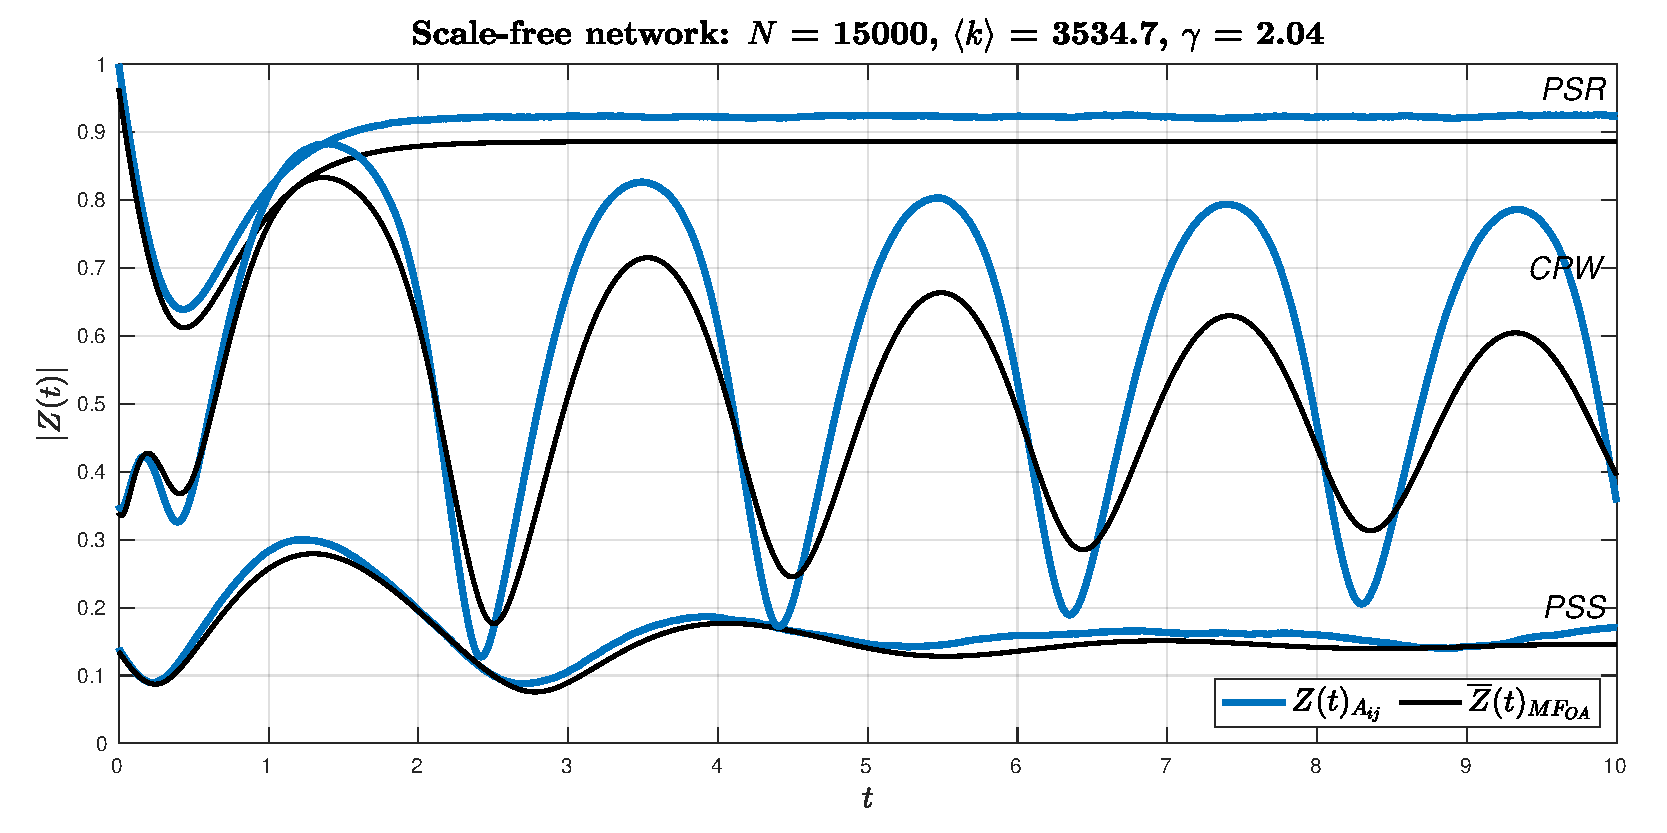
\includegraphics[width = \textwidth]{../Figures/InspectMeanFieldScaleFree.pdf}
\caption{Comparison of the simulation of a scale-free network of Theta neurons and the Ott-Antonsen theory by the magnitude of the order parameter.}
\label{fig:InspectMeanFieldScaleFree}
\end{figure}

\begin{figure}[H]
\centering
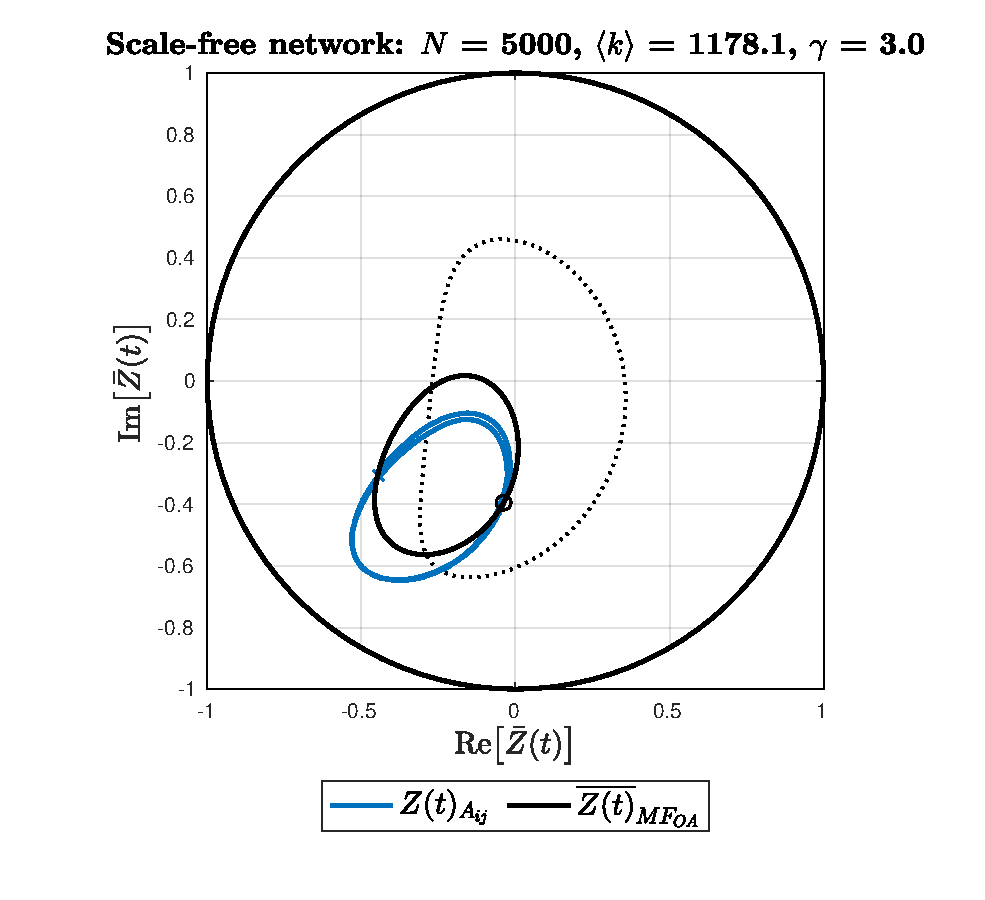
\includegraphics[width = 0.75\textwidth]{../Figures/PhaseSpace/InspectMeanFieldScaleFreePhaseSpace.pdf}
\caption{Comparison of the limit cycles found by theory and simulation.}
\label{fig:InspectMeanFieldScaleFreePhaseSpace}
\end{figure}


